\documentclass[man,a4paper,12pt,floatsintext,nolmodern,notab]{apa7}
\usepackage[american]{babel}
\usepackage{fontspec}
\setmainfont{TeX Gyre Termes}
\setsansfont{TeX Gyre Heros}
\newfontfamily\cjkfont{HaranoAjiMincho-Regular.otf}
\usepackage{graphicx}
\usepackage{booktabs}
\usepackage{array}
\usepackage{xurl}
\urlstyle{same}
\hypersetup{hidelinks}
\usepackage{longtable}
\usepackage{needspace}
\usepackage{setspace}
\usepackage{microtype}
\newcommand{\tablefont}{\small}

\title{Effects of Unplugged Activities on Computational Thinking in School Students: A Meta-Analysis}
\shorttitle{EFFECTS OF UNPLUGGED ACTIVITIES ON COMPUTATIONAL}
\authorsnames{Society for Educational Data Analysis (SEDA)}
\authorsaffiliations{Generative AI paper}
\abstract{Developing computational thinking skills in early education is increasingly vital, prompting schools to explore diverse pedagogical approaches. Using an automated workflow in which every extracted number was verified against the full text, 6 open-access studies (\textit{N} = 450) were pooled with a random-effects model. The pooled effect was \textit{g} = 0.51, 95\% CI [\ensuremath{-}0.15, 1.16], with \textit{I}² = 80.9\%. Unplugged activities show moderate potential for fostering computational thinking, but further rigorous research is required to confirm their effectiveness in primary and lower secondary classrooms.}
\keywords{meta-analysis, unplugged activities, computational thinking, elementary education, computer science education}
\authornote{This is a “Generative AI paper” produced automatically by the Society for Educational Data Analysis (SEDA) with generative AI. Large language models (gemini-3.6-flash, gemini-3.8-flash, gemini-3.5-flash, gemini-3.5-flash-lite) were used to screen records, extract data, and draft the Introduction, Discussion, and Conclusion; all statistics were computed by software. The paper has not been peer reviewed.

The Japanese version of this paper, with identical content, is available at \url{https://raw.githubusercontent.com/k518-2026/MetaAnalysisToWP/main/reports/2026-10-04-info-unplugged-ct/paper-ja.pdf}. Published October 4, 2026.

Data and code are available at \url{https://github.com/k518-2026/MetaAnalysisToWP}. © 2026 Society for Educational Data Analysis (SEDA).}
\begin{document}
\maketitle
Primary and lower secondary schools are increasingly integrating computer science concepts into their curricula to prepare students for a digital world. Developing computational thinking at an early age is considered essential for fostering problem-solving and logical reasoning skills. However, schools often face resource constraints, such as a lack of computers or internet access, which can hinder the implementation of digital programming lessons.

To address these challenges, educators have turned to unplugged (computer-free) computer science and computational thinking activities. These activities use physical games, puzzles, cards, or kinesthetic movements to teach core concepts like algorithms, patterns, and debugging without requiring digital devices. Researchers have investigated various unplugged approaches, including general computational thinking activities (Brackmann et al., 2019; Montes-León et al., 2020), coding tasks (Namlı \& Aybek, 2022), specific tools like Tospaa (Yilmaz \& İzmirli, 2023), musical activities based on Bebras challenges (Durán et al., 2023), and educational board games like SmartGames (Fanchamps et al., 2023).

While individual studies report positive or mixed outcomes, their findings are often limited by small sample sizes and diverse comparison groups, which range from regular lessons (Montes-León et al., 2020; Namlı \& Aybek, 2022) and no computational thinking instruction (Brackmann et al., 2019; Durán et al., 2023) to plugged-in programming (Fanchamps et al., 2023; Yilmaz \& İzmirli, 2023). A quantitative synthesis is useful to systematically pool these disparate findings, estimate the overall effect size, and evaluate the consistency of unplugged activities across different educational contexts.

The purpose of this meta-analysis is to synthesize the existing empirical evidence on the effectiveness of unplugged activities. Specifically, this study addresses the following research question: What is the overall effect of unplugged computer science and computational thinking activities on the computational thinking test performance of school students compared to control conditions?

\section{Method}
\subsection{Literature Search}
Searches were run on October 4, 2026 in two open bibliographic sources. OpenAlex was searched in the title and abstract fields with the query “(unplugged) AND (“computational thinking” OR programming OR “computer science”) AND (elementary OR primary OR “middle school” OR “junior high” OR secondary OR “K-12” OR grade OR children OR pupils)”, restricted to open-access journal articles published in 2012 or later and classified in the Education or Developmental and Educational Psychology subfields. J-STAGE, the Japanese journal platform, was searched in the abstract field with the keywords “{\cjkfont アンプラグド} {\cjkfont プログラミング}”, “{\cjkfont アンプラグド} {\cjkfont 小学校}” (2012 or later) to include studies published in Japan.

\subsection{Eligibility Criteria}
Studies were eligible if they (a) sampled students in primary or secondary school (K-12); Primary and lower secondary samples are preferred; upper secondary samples are acceptable; Exclude university, adult, and teacher/pre-service teacher samples; (b) examined unplugged (computer-free) computer science or computational thinking activities; (c) compared it with no computational thinking instruction, regular lessons, or plugged (computer-based) activities; (d) measured a computational thinking test or programming concept test; and (e) reported statistics sufficient to compute a standardized mean difference. Reviews, qualitative studies, single-case designs, and single-group pre-post designs were excluded.

\subsection{Screening and Data Extraction}
Screening and data extraction were automated. A large language model (gemini-3.6-flash, gemini-3.8-flash, gemini-3.5-flash, gemini-3.5-flash-lite) rated each title and abstract against the eligibility criteria. Full texts (PDF) of the highest-rated records were retrieved and converted to plain text, and the model extracted study characteristics and summary statistics from them. Every extracted number was then checked by software against the full text, and a study was excluded from the synthesis if any extracted number could not be found verbatim. No human reviewer verified the screening or the extraction. When more than 10 studies qualified, the 10 with the highest screening ratings were retained.

\subsection{Effect Sizes}
Standardized mean differences were computed as Hedges’ g (Hedges, 1981) from post-test means, standard deviations, and group sizes; when these were unavailable, from independent-samples t statistics, from F statistics with one numerator degree of freedom, or from reported d or g values. Positive values indicate higher scores in the intervention group. One effect size per study was used.

\subsection{Statistical Analysis}
Effect sizes were pooled with a random-effects model in which the between-study variance (\textit{τ}²) was estimated with the DerSimonian–Laird method (DerSimonian \& Laird, 1986). Confidence intervals and tests of the pooled effect used the Hartung–Knapp–Sidik–Jonkman (HKSJ) adjustment, which is recommended when the number of studies is small (Hartung \& Knapp, 2001; IntHout et al., 2014). Heterogeneity was assessed with Q, \textit{I}² (Higgins \& Thompson, 2002), \textit{τ}², and a 95\% prediction interval. Subgroup analyses by school level (elementary: grades 1–6; lower secondary: grades 7–9) were conducted when each level included at least two studies. Robustness was examined with leave-one-out analysis, and Egger’s regression test (Egger et al., 1997) was planned only when at least 10 studies were available. Effect magnitudes were interpreted with conventional benchmarks (Cohen, 1988). Analyses followed standard formulas (Borenstein et al., 2009) implemented in open-source JavaScript code (\url{https://github.com/k518-2026/MetaAnalysisToWP}).

\section{Results}
\subsection{Study Selection}
The searches returned 189 records from OpenAlex (of 189 matching the query) and 18 from J-STAGE, for 204 unique records. Of the 194 records with abstracts that were screened, 21 were rated as potentially eligible. Full texts of 21 records were examined: 6 could not be retrieved or read, 5 did not meet the eligibility criteria, 3 did not report sufficient statistics, 1 contained extracted numbers that could not be verified in the text, and 0 yielded implausible values. In total, 6 studies were included in the meta-analysis.

\subsection{Study Characteristics}
Table 1 summarizes the country, grade, design, sample size, and effect size of each included study (Brackmann et al., 2019; Durán et al., 2023; Fanchamps et al., 2023; Montes-León et al., 2020; Namlı \& Aybek, 2022; Yilmaz \& İzmirli, 2023). The studies comprised 450 participants in total and were conducted in Ecuador, Turkey, Spain, Netherlands, Brazil. By school level, 1 study sampled other students, 4 studies sampled elementary (grades 1–6) students, 1 study sampled lower secondary (grades 7–9) students. Sample sizes ranged from 22 to 220, and individual effect sizes ranged from \textit{g} = \ensuremath{-}0.64 to \textit{g} = 1.33.

\par\vspace{4pt}
{\tablefont\singlespacing\setlength{\LTpre}{6pt}\setlength{\LTpost}{2pt}
\begin{longtable}{>{\raggedright\arraybackslash}p{0.2600\dimexpr\linewidth-12\tabcolsep\relax}>{\raggedright\arraybackslash}p{0.1100\dimexpr\linewidth-12\tabcolsep\relax}>{\raggedright\arraybackslash}p{0.1200\dimexpr\linewidth-12\tabcolsep\relax}>{\raggedright\arraybackslash}p{0.2300\dimexpr\linewidth-12\tabcolsep\relax}>{\raggedright\arraybackslash}p{0.0700\dimexpr\linewidth-12\tabcolsep\relax}>{\raggedright\arraybackslash}p{0.2100\dimexpr\linewidth-12\tabcolsep\relax}}
\multicolumn{6}{@{}l@{}}{\textbf{Table 1}} \\
\multicolumn{6}{@{}p{\linewidth}@{}}{\textit{Overview of the Included Studies}} \\[3pt]
\toprule
Study & Country & Grade & Design & \textit{N} & \textit{g} [95\% CI] \\
\midrule
\endfirsthead
\toprule
Study & Country & Grade & Design & \textit{N} & \textit{g} [95\% CI] \\
\midrule
\endhead
Montes-León et al. (2020) & Ecuador & Grade 10 & quasi-experimental & 80 & 0.69 [0.25, 1.14] \\
Namlı and Aybek (2022) & Turkey & Grade 5 & randomized controlled trial & 54 & 0.37 [\ensuremath{-}0.17, 0.90] \\
Yilmaz and İzmirli (2023) & Turkey & Grade 5 & quasi-experimental & 36 & 0.56 [\ensuremath{-}0.09, 1.22] \\
Durán et al. (2023) & Spain & Grades 3-6 & quasi-experimental & 220 & 1.33 [1.00, 1.67] \\
Fanchamps et al. (2023) & Netherlands & Grades 5-6 & randomized controlled trial & 22 & \ensuremath{-}0.64 [\ensuremath{-}1.47, 0.19] \\
Brackmann et al. (2019) & Brazil & Grades 5-6 & quasi-experimental & 38 & 0.36 [\ensuremath{-}0.27, 0.98] \\
\bottomrule
\end{longtable}
\noindent \textit{Note.} CI = confidence interval. \textit{g} = Hedges’ g (positive values favor the intervention). Grades and designs were extracted automatically from the full texts.\par}
\vspace{6pt}
Table 2 lists the intervention, comparison condition, and outcome measure of each study. All 6 studies compared an intervention group with a comparison group on a post-test.

\par\vspace{4pt}
{\tablefont\singlespacing\setlength{\LTpre}{6pt}\setlength{\LTpost}{2pt}
\begin{longtable}{>{\raggedright\arraybackslash}p{0.2000\dimexpr\linewidth-8\tabcolsep\relax}>{\raggedright\arraybackslash}p{0.3200\dimexpr\linewidth-8\tabcolsep\relax}>{\raggedright\arraybackslash}p{0.2400\dimexpr\linewidth-8\tabcolsep\relax}>{\raggedright\arraybackslash}p{0.2400\dimexpr\linewidth-8\tabcolsep\relax}}
\multicolumn{4}{@{}l@{}}{\textbf{Table 2}} \\
\multicolumn{4}{@{}p{\linewidth}@{}}{\textit{Interventions, Comparison Conditions, and Outcome Measures}} \\[3pt]
\toprule
Study & Intervention & Comparison & Outcome \\
\midrule
\endfirsthead
\toprule
Study & Intervention & Comparison & Outcome \\
\midrule
\endhead
Montes-León et al. (2020) & unplugged computational thinking activities & regular logical and mathematical reasoning instruction & computational thinking test \\
Namlı and Aybek (2022) & unplugged coding activities & regular curriculum instruction without interventions & International Informatics and Computational Thinking Activity Task Test \\
Yilmaz and İzmirli (2023) & Tospaa unplugged coding activities & Scratch block-based coding activities & Computational Thinking Test \\
Durán et al. (2023) & unplugged musical activities based on Bebras challenges & no computational thinking instruction & Computational Thinking Test using Bebras Problems \\
Fanchamps et al. (2023) & unplugged SmartGames & plugged-in sense-reason-act programming using Lego EV-3 & Computational Thinking Test \\
Brackmann et al. (2019) & unplugged computational thinking activities & no computational thinking instruction & Computational Thinking Test \\
\bottomrule
\end{longtable}
\noindent \textit{Note.} Extracted and summarized automatically from the full texts.\par}
\vspace{6pt}
\subsection{Overall Effect}
Figure 1 shows the forest plot. Each square marks the effect size of one study, with its size proportional to the study’s weight, and each horizontal line marks the 95\% confidence interval; the diamond at the bottom is the pooled estimate. 5 of the 6 studies had positive effect sizes, and the confidence intervals of 2 studies did not include zero. The study with the largest weight was Durán et al. (2023) (19.5\%).

\begin{figure}[!htbp]
\caption{Forest Plot of Individual and Pooled Effect Sizes}
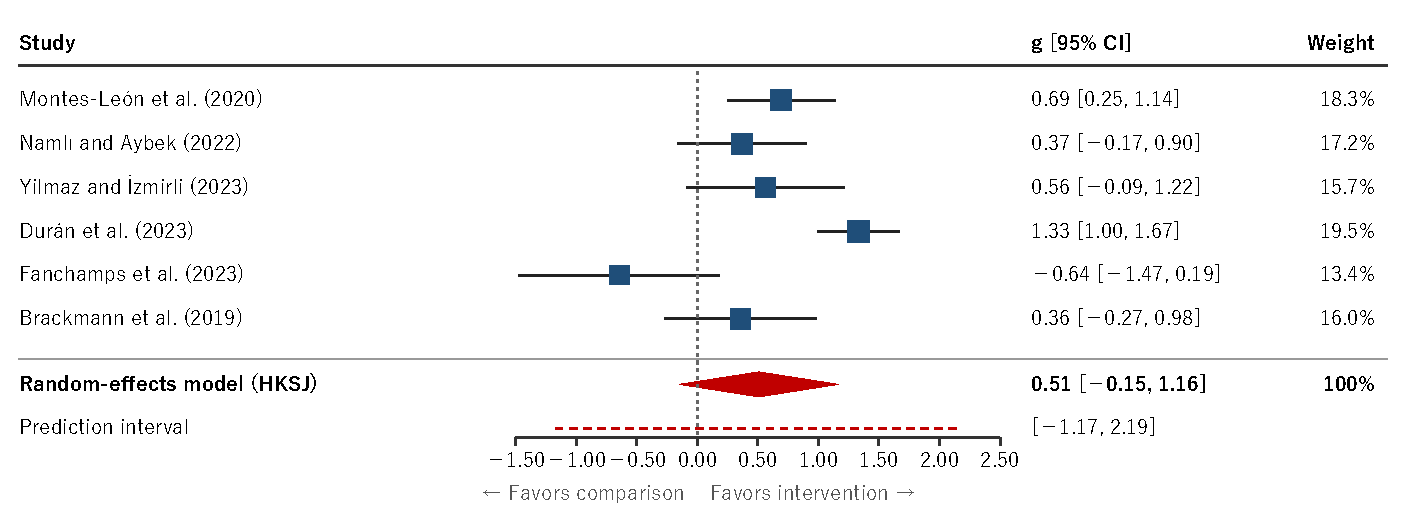
\includegraphics[width=\linewidth]{forest-en.pdf}
\figurenote{Squares show study effect sizes (size proportional to weight), lines show 95\% confidence intervals, the diamond shows the pooled estimate, and the dashed line shows the prediction interval.}
\end{figure}
The random-effects model yielded a pooled effect of \textit{g} = 0.51, 95\% CI [\ensuremath{-}0.15, 1.16], \textit{t}(5) = 2.00, \textit{p} = .103, which is not statistically significant: the confidence interval includes zero, so the data are also compatible with no effect, although the point estimate corresponds to a moderate effect by conventional benchmarks. The fixed-effect estimate was \textit{g} = 0.75. Table 3 summarizes these estimates.

\subsection{Heterogeneity}
Heterogeneity was considerable, \textit{Q}(5) = 26.13, p < .001, \textit{I}² = 80.9\%, \textit{τ}² = 0.302. The 95\% prediction interval ranged from \ensuremath{-}1.17 to 2.19.

\subsection{Subgroup and Sensitivity Analyses}
A subgroup analysis by school level was not conducted because fewer than two studies were available for at least one level. Leave-one-out estimates ranged from 0.35 to 0.70. Publication bias was not tested because fewer than 10 studies were included.

\par\vspace{4pt}
{\tablefont\singlespacing\setlength{\LTpre}{6pt}\setlength{\LTpost}{2pt}
\begin{longtable}{lrrrrrrr}
\multicolumn{8}{@{}l@{}}{\textbf{Table 3}} \\
\multicolumn{8}{@{}p{\linewidth}@{}}{\textit{Results of the Meta-Analysis}} \\[3pt]
\toprule
Model & \textit{k} & \textit{N} & \textit{g} & 95\% CI & \textit{p} & \textit{I}² (\%) & \textit{τ}² \\
\midrule
\endfirsthead
\toprule
Model & \textit{k} & \textit{N} & \textit{g} & 95\% CI & \textit{p} & \textit{I}² (\%) & \textit{τ}² \\
\midrule
\endhead
Random effects (HKSJ) & 6 & 450 & 0.51 & [\ensuremath{-}0.15, 1.16] & .103 & 80.9 & 0.302 \\
Fixed effect & 6 & 450 & 0.75 & [0.55, 0.96] & < .001 & — & — \\
\bottomrule
\end{longtable}
\noindent \textit{Note.} \textit{k} = number of studies. HKSJ = Hartung–Knapp–Sidik–Jonkman confidence interval. 95\% prediction interval [\ensuremath{-}1.17, 2.19].\par}
\vspace{6pt}
\section{Discussion}
The meta-analysis pooled data from 6 studies with a total sample size of 450 students. As shown in Table 3, the overall pooled effect size was moderate, with Hedges \textit{g} = 0.51, but this effect was not statistically significant (95\% CI [-0.15, 1.16], \textit{p} = .103). The forest plot (Figure 1) reveals substantial heterogeneity among the included studies, as indicated by \textit{Q}(5) = 26.13, p < .001, I2 = 80.9\%, and tau2 = 0.302. This high level of heterogeneity suggests that the effectiveness of unplugged activities varies considerably depending on the specific implementation and context. The wide prediction interval of [-1.17, 2.19] further highlights that future implementations could result in either highly positive or negative outcomes.

To assess the robustness of the pooled estimate, a leave-one-out sensitivity analysis was conducted, yielding a range of pooled Hedges g from 0.35 to 0.70, indicating that no single study disproportionately dictated the direction of the overall effect. Subgroup analyses based on school levels were not conducted because there were fewer than 2 studies per school level, preventing a reliable comparison. Additionally, publication bias was not assessed due to the small number of included studies (fewer than 10).

An overview of the studies is presented in Table 1, and the specific interventions and outcomes are detailed in Table 2. The individual study effects varied widely. For instance, (Durán et al., 2023) reported a very large positive effect (\textit{g} = 1.33) for unplugged musical activities based on Bebras challenges compared to no instruction. Moderate positive effects were observed in quasi-experimental designs, such as (Montes-León et al., 2020) in Ecuador (\textit{g} = 0.69) and (Yilmaz \& İzmirli, 2023) in Turkey (\textit{g} = 0.56). In contrast, (Fanchamps et al., 2023) found a negative effect (\textit{g} = -0.64) when comparing unplugged SmartGames to plugged-in Lego EV-3 programming, although the authors noted equivalent development. Other studies, such as (Namlı \& Aybek, 2022) (\textit{g} = 0.37) and (Brackmann et al., 2019) (\textit{g} = 0.36), showed smaller, non-significant positive trends.

For teachers of grades 1-9, these findings suggest that unplugged activities can be a viable, low-cost entry point for teaching computational thinking, especially when digital resources are scarce. However, because the overall effect was not statistically significant and highly variable, teachers should not view unplugged activities as a complete replacement for plugged-in programming. Instead, integrating unplugged lessons with physical or musical elements, as seen in (Durán et al., 2023), or combining them with block-based programming (Namlı \& Aybek, 2022; Yilmaz \& İzmirli, 2023) may yield the most balanced educational outcomes.

\section{Conclusion}
In conclusion, this meta-analysis indicates that unplugged computer science activities have a moderate but statistically non-significant overall effect (\textit{g} = 0.51) on students' computational thinking skills. The high heterogeneity and wide prediction interval underscore the diverse outcomes of these interventions in practice. While unplugged activities offer a promising, accessible tool for primary and lower secondary school teachers, further rigorous, large-scale research is essential to identify the specific conditions and designs that maximize their effectiveness.

Several limitations must be acknowledged when interpreting these results. First, the meta-analysis is based on a very small number of studies (6 studies, \textit{N} = 450), which limits the statistical power to detect a significant overall effect and prevents robust subgroup or publication bias analyses. Second, the data were extracted automatically, which may introduce minor inaccuracies or overlook nuanced contextual details.

Additionally, the included studies employed diverse research designs, ranging from randomized controlled trials (Fanchamps et al., 2023; Namlı \& Aybek, 2022) to quasi-experimental designs (Brackmann et al., 2019; Durán et al., 2023; Montes-León et al., 2020; Yilmaz \& İzmirli, 2023). The outcome measures also varied, utilizing different computational thinking tests, such as Bebras tasks (Durán et al., 2023) or general computational thinking tests (Brackmann et al., 2019; Fanchamps et al., 2023; Montes-León et al., 2020; Yilmaz \& İzmirli, 2023), which may not capture the same underlying constructs. Finally, the samples were predominantly focused on elementary grades (Brackmann et al., 2019; Durán et al., 2023; Fanchamps et al., 2023; Namlı \& Aybek, 2022; Yilmaz \& İzmirli, 2023), with only one study targeting grade 10 (Montes-León et al., 2020), limiting the generalizability of the findings across all K-12 school levels.

In addition, screening and data extraction were automated with a language model, and extracted numbers were verified only by matching them against the full text. A number can be present in the text yet belong to a different group or measure. Only open-access studies whose full texts could be retrieved were included; subscription-only and unpublished studies were not.

\section{References}
\noindent References marked with an asterisk indicate studies included in the meta-analysis.\par
\par\noindent\hangindent=0.5in\hangafter=1 Borenstein, M., Hedges, L. V., Higgins, J. P. T., \& Rothstein, H. R. (2009). \textit{Introduction to meta-analysis}. Wiley. \url{https://doi.org/10.1002/9780470743386}\par
\par\noindent\hangindent=0.5in\hangafter=1 *Brackmann, C. P., Barone, D. A. C., Boucinha, R. M., \& Reichert, J. T. (2019). Development of computational thinking in Brazilian schools with social and economic vulnerability. \textit{International Journal for Innovation Education and Research}, \textit{7}(4), 79–96. \url{https://doi.org/10.31686/ijier.vol7.iss4.1390}\par
\par\noindent\hangindent=0.5in\hangafter=1 Cohen, J. (1988). \textit{Statistical power analysis for the behavioral sciences} (2nd ed.). Lawrence Erlbaum Associates.\par
\par\noindent\hangindent=0.5in\hangafter=1 DerSimonian, R., \& Laird, N. (1986). Meta-analysis in clinical trials. \textit{Controlled Clinical Trials}, \textit{7}(3), 177–188. \url{https://doi.org/10.1016/0197-2456(86)90046-2}\par
\par\noindent\hangindent=0.5in\hangafter=1 *Durán, C. M. S., García-Fernández, C. M., \& Galán, A. A. (2023). Alfabetización Computacional: Actividades musicales desenchufadas sobre el Desafío Internacional de Bebras. \textit{Revista de Educación a Distancia (RED)}, \textit{23}(73). \url{https://doi.org/10.6018/red.540191}\par
\par\noindent\hangindent=0.5in\hangafter=1 Egger, M., Davey Smith, G., Schneider, M., \& Minder, C. (1997). Bias in meta-analysis detected by a simple, graphical test. \textit{BMJ}, \textit{315}(7109), 629–634. \url{https://doi.org/10.1136/bmj.315.7109.629}\par
\par\noindent\hangindent=0.5in\hangafter=1 *Fanchamps, N. L. J. A., van Gool, E., Slangen, L., \& Hennissen, P. (2023). The effect on computational thinking and identified learning aspects: Comparing unplugged smartGames with SRA-Programming with tangible or On-screen output. \textit{Education and Information Technologies}, \textit{29}(3), 2999–3024. \url{https://doi.org/10.1007/s10639-023-11956-6}\par
\par\noindent\hangindent=0.5in\hangafter=1 Hartung, J., \& Knapp, G. (2001). A refined method for the meta-analysis of controlled clinical trials with binary outcome. \textit{Statistics in Medicine}, \textit{20}(24), 3875–3889. \url{https://doi.org/10.1002/sim.1009}\par
\par\noindent\hangindent=0.5in\hangafter=1 Hedges, L. V. (1981). Distribution theory for Glass's estimator of effect size and related estimators. \textit{Journal of Educational Statistics}, \textit{6}(2), 107–128. \url{https://doi.org/10.3102/10769986006002107}\par
\par\noindent\hangindent=0.5in\hangafter=1 Higgins, J. P. T., \& Thompson, S. G. (2002). Quantifying heterogeneity in a meta-analysis. \textit{Statistics in Medicine}, \textit{21}(11), 1539–1558. \url{https://doi.org/10.1002/sim.1186}\par
\par\noindent\hangindent=0.5in\hangafter=1 IntHout, J., Ioannidis, J. P. A., \& Borm, G. F. (2014). The Hartung-Knapp-Sidik-Jonkman method for random effects meta-analysis is straightforward and considerably outperforms the standard DerSimonian-Laird method. \textit{BMC Medical Research Methodology}, \textit{14}, Article 25. \url{https://doi.org/10.1186/1471-2288-14-25}\par
\par\noindent\hangindent=0.5in\hangafter=1 *Montes-León, H., Neira, R. H., Pérez-Marín, D., \& León, S. R. M. (2020). Improving computational thinking in secondary students with unplugged tasks. \textit{Education in the Knowledge Society (EKS)}, \textit{21}, 12. \url{https://doi.org/10.14201/eks.23002}\par
\par\noindent\hangindent=0.5in\hangafter=1 *Namlı, N. A., \& Aybek, B. (2022). An investigation of the effect of block-based programming and unplugged coding activities on fifth graders’ computational thinking skills, self-efficacy and academic performance. \textit{Contemporary Educational Technology}, \textit{14}(1), ep341. \url{https://doi.org/10.30935/cedtech/11477}\par
\par\noindent\hangindent=0.5in\hangafter=1 *Yilmaz, T., \& İzmirli, S. (2023). Effect of unplugged and plugged coding activities on secondary school students’ computational thinking skills. \textit{Journal of Educational Technology and Online Learning}, \textit{6}(4), 1180–1193. \url{https://doi.org/10.31681/jetol.1375335}\par
\end{document}
